\documentclass[12pt,utf8]{beamer}
\setbeamercovered{transparent}
\usepackage[german]{babel}
\usepackage{color}
\usepackage{xcolor}
\usepackage{graphicx}
\usepackage{tikz}
\usetheme{FOSSAG}

\title{Linux Basics}
\subtitle{Das Terminal}


\author[J.-M. Lenk, C. Parnitzke, Y. Bungers, A. Becker]{Jan-Marius Lenk, Christoph Parnitzke, Yannick Bungers, Alexander Becker}
\institute[FOSS AG]{Free and Open Source Software AG\\ Fakultät für Informatik}

\date{\today}

\begin{document}

\titlepage

\begin{frame}
\frametitle{Inhaltsverzeichnis}
\begin{itemize}
	\item Einleitung
	\item Arbeiten mit Ordnern, Dateien und Archiven
	\item Systemverwaltung
\end{itemize}
\end{frame}

\section{Einleitung}
\begin{frame}
\frametitle{Unix Philosophie}
\begin{figure}

\includegraphics[scale=0.15]{res/tuX_tu.png}
\end{figure}
\begin{itemize}
	\item Philosophie besteht aus drei Punkten:
	\begin{itemize}
		\item 1. Schreibe Programme, die nur eine Sache tun und dies erfolgreich
		\item 2. Schreibe Programme, die Kolaboration ermöglichen
		\item 3. Schreibe Programme, die mit Text arbeiten, denn dies ist universell
	\end{itemize}
\end{itemize}
%\footnote{https://upload.wikimedia.org/wikipedia/commons/a/af/Tux.png}
\end{frame}

\section{Arbeiten mit Ordnern, Dateien und Archiven}
\subsection{Ordner}
\begin{frame}
	\frametitle{\textcolor{lightGreen}{l}i\textcolor{lightGreen}{s}t}
	\framesubtitle{Ein kleines Licht in der Dunkelheit}
	\begin{itemize}
		\item Listet alle Ordner und Dateien in Verzeichnis auf
		\item Mögliche Optionen:
		\begin{itemize}[<+->]
			\item \texttt{-a}  (all) inkl. versteckter Verzeichnisse
			\item \texttt{-hl}  (human readable / long listing format) inkl. Rechte, Besitzer, Größe, etc.
		\end{itemize}
	\end{itemize}
\end{frame}

\begin{frame}
	\frametitle{\textcolor{lightGreen}{c}hange \textcolor{lightGreen}{d}irectory}
	\framesubtitle{Die kleine Form der Teleportation}
	\texttt{cd} ermöglicht das Navigieren durch das Dateisystem
	\begin{itemize}
		\item Wechsel in Parent-Directory mit \texttt{cd ..}
		\item Wechsel in Home-Directory mit \texttt{cd} ($\sim$)
	\end{itemize}
\end{frame}

\begin{frame}
\frametitle{\textcolor{lightGreen}{c}o\textcolor{lightGreen}{p}y $\&$ \textcolor{lightGreen}{m}o\textcolor{lightGreen}{v}e}
\framesubtitle{Die Kunst des Klonens und Umbenennens}
\begin{itemize}
	\item \texttt{mv PATH1 PATH2} (Verschieben von Dateien/Ordnern)
	\item \texttt{cp PATH1 PATH2} (Kopieren von Dateien)
	\begin{itemize}
		\item -r ermöglicht kopieren von Ordnern
	\end{itemize}
\end{itemize}
\end{frame}

\begin{frame}
\frametitle{\textcolor{lightGreen}{m}a\textcolor{lightGreen}{k}e \textcolor{lightGreen}{dir}ectory}
\framesubtitle{Verzeichnisse erschaffen}
\texttt{mkdir} erstellt Ordner auf dem Rechner
\begin{itemize}
	\item \texttt{mkdir PATH}
	\item \texttt{-p} erstellt alle Ordner auf dem Pfad, die noch nicht existieren
\end{itemize}
\end{frame}

\begin{frame}
\frametitle{\textcolor{lightGreen}{r}e\textcolor{lightGreen}{m}ove}
\framesubtitle{Flutsch! Und weg!}
\begin{itemize}
	\item \texttt{rm [OPTION] FILE}
	\begin{itemize}[<+->]
		\item \texttt{-r} ermöglicht das Löchen von Ordnern
	\end{itemize}
\end{itemize}
\end{frame}

\begin{frame}
	\frametitle{find}
	\texttt{find} sucht Dateien im aktuellen Ordner und in Unterordnern
	\begin{itemize}
		\item \texttt{find -name FILE}
	\end{itemize}
\end{frame}

\subsection{Archive}
\begin{frame}
\frametitle{\textcolor{lightGreen}{t}ape \textcolor{lightGreen}{ar}chiver}
\framesubtitle{Archivieren}
Zum entpacken von Archiven wie \texttt{.tar}, \texttt{.tar.gz}, \texttt{.zip}, etc. 
\begin{itemize}
	\item \texttt{tar -czvf ARCHIVE\_PATH PATH\_FILES}\\(Verpacken)
	\item \texttt{tar -xzvf ARCHIVE\_PATH}\\(Entpacken)
\end{itemize}
\end{frame}

\begin{frame}
\frametitle{\Large{\textcolor{lightGreen}{g}lobally search a \textcolor{lightGreen}{r}egular \textcolor{lightGreen}{e}xpression and \textcolor{lightGreen}{p}rint}}
\framesubtitle{Gonna catch em' Strings}
\texttt{grep} ermöglicht die Suche in einer Eingabe
\begin{itemize}
	\item \texttt{-i} ignoriert Groß- und Kleinschreibung bei der Suche
\end{itemize}
\end{frame}

\begin{frame}
\frametitle{man page}
\framesubtitle{Wenn man mal nicht weiter weiß}
Anleitungen (Manuals) zu den installierten Paketen lassen sich mit \texttt{man} betrachten.
\begin{itemize}
	\item man COMMAND
\end{itemize}
\end{frame}

\begin{frame}
\frametitle{\textcolor{lightGreen}{t}ape \textcolor{lightGreen}{ar}chiver}
\framesubtitle{Archivieren}
\begin{itemize}[<+->]
\item {\scriptsize \texttt{-c} (create) erzeugt neues Archiv}
\item {\scriptsize \texttt{-x} (extract) extrahieren einer Datei}
\item {\scriptsize \texttt{-v} (verbose) Fortschritt auflisten}
\item {\scriptsize \texttt{-z} (gzip format) komprimieren als \texttt{.gz}, etc.}
\item {\scriptsize \texttt{-f} erzeugt beim Entpacken einen Ordner mit Namen von Archiv}
\end{itemize}
\end{frame}

\begin{frame}
\frametitle{\Large Dateien betrachten und bearbeiten}
\begin{itemize}
	\item \texttt{cat FILE} - Ausgabe einer Datei
	\item \texttt{less FILE} - Betrachten einer Datei
	\item \texttt{nano FILE} - Bearbeiten einer Datei
\end{itemize}
\end{frame}

\subsection{Dateien}
\begin{frame}
	\centering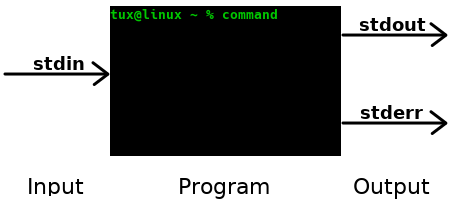
\includegraphics[scale=0.65]{res/IOE}
\end{frame}

\begin{frame}
	\Huge\centering{$|$~~~$>$}
\end{frame}

\begin{frame}
\Huge\centering{\&}
\end{frame}

\section{Systemverwaltung}
\subsection{Prozesse verwalten}
\begin{frame}
\frametitle{\textcolor{lightGreen}{h}isham \textcolor{lightGreen}{t}able \textcolor{lightGreen}{o}f \textcolor{lightGreen}{p}rocesses}
\framesubtitle{interaktiver Prozessager}
\begin{itemize}
	\item \texttt{\textcolor{red}{t}able \textcolor{red}{o}f \textcolor{red}{p}rocesses} (bereits installtiert)
	\item \texttt{htop} (muss installiert werden)
	\begin{itemize}[<+->]
		\item {\scriptsize Übersicht über alle Prozesse und verbrauchte Ressourcen}
		\item {\scriptsize deutlich leichtere Bedienung und bessere Übersicht}
		\item {\scriptsize bietet mehr Interaktionen}
	\end{itemize}
\end{itemize}
\end{frame}

\subsection{Paketverwaltung}
\begin{frame}
	\frametitle{\textcolor{lightGreen}{s}uper \textcolor{lightGreen}{u}ser \textcolor{lightGreen}{do}}
	\framesubtitle{Mit großer Macht kommt große Verantwortung}
	\texttt{sudo} führt einen Befehl mit administrativer Berechtigung aus
	\begin{itemize}
		\item \texttt{sudo COMMAND}
	\end{itemize}
\end{frame}

\begin{frame}
	\frametitle{apt}
	Mit \texttt{apt} lassen sich Pakete installieren und deinstallieren
	\begin{itemize}
		\item \texttt{sudo apt install PACKAGE}
		\item \texttt{sudo apt update}
		\item \texttt{sudo apt upgrade / dist-upgrade}
		\item \texttt{sudo apt remove PACKAGE}
		\item \texttt{sudo apt search PACKAGE}
	\end{itemize}
\end{frame}

\subsection{Herunterfahren und Neustarten}
\begin{frame}
\frametitle{poweroff und reboot}
\framesubtitle{Wenn man mal das real life genießen will}
\begin{itemize}
	\item \texttt{poweroff} (Herunterfahren des Systems)
	\item \texttt{reboot} (Neustart des Systems)
\end{itemize}
\end{frame}


\end{document}
